%!TEX root = ./thesis.tex

\chapter{Hardware implementation}
\label{cha:hard}

A hardware implementation consist in a set of file written in \gls{hdl} with constraints associated to these files. First, I describe the hardware implementation of operations on posit numbers, which are the basic building blocks of \glspl{spn}. Then I explain how \glspl{spn} hardware files are generated from a trained \gls{spn} file. Finally, I describe the implementation of the \gls{spn} inside the \gls{fpga} with the complete control scheme. The design is intended to work on a Zed Board.

% ==============================================================================
\section{Posit representation}
% ==============================================================================

In this section, I describe how posit operations are performed in hardware. The general schematic is described in Figure \ref{fig:posit_op}. The floating point operation mentioned here represents the operation described in Algorithm \ref{alg:float_add} and \ref{alg:float_mult}. For a posit operation, the size of each field must be properly computed and is different from a classical floating point operation.

\begin{figure}[!ht]
\begin{mdframed}
	\centering
	\includestandalone[width=\linewidth]{../Images/operator}
	\caption{Illustration for posit operations}
	\label{fig:posit_op}
\end{mdframed}
\end{figure}

% ------------------------------------------------------------------------------
\subsection{Encoder and Decoder}
% ------------------------------------------------------------------------------
As posit representation use variable size fields, an encoder and decoder are required to extract useful information from a raw binary sequence.

The encoder schematized in Figure \ref{fig:enc_mod} is composed of two smaller encoder. A first one which convert an exponent into a regime value and an exponent value. And a second one which take as input the regime, the exponent and the significand to output a posit number. It is in this block that the number are truncated in case of rounding and that information is lost.

The decoder schematized in Figure \ref{fig:dec_mod} is basically the inverse of the encoder except that there is no rounding implemented.

\begin{figure}[!ht]
\begin{mdframed}
	\subfloat[Encoder]{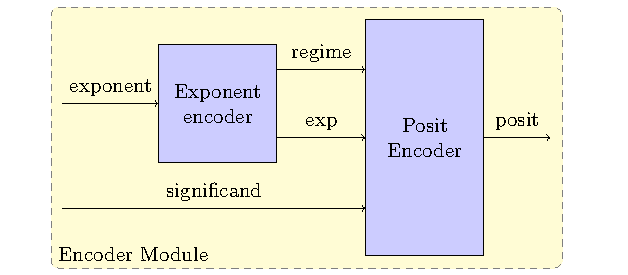
\includegraphics[width=0.49\linewidth]{../Images/encoder_module} \label{fig:enc_mod}}
	\subfloat[Decoder]{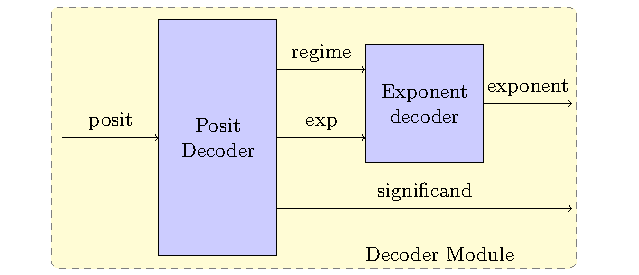
\includegraphics[width=0.49\linewidth]{../Images/decoder_module} \label{fig:dec_mod}}
	\caption{Schematic of encoder and decoder modules}
	\label{fig:enc_dec_mod}
\end{mdframed}
\end{figure}

% ------------------------------------------------------------------------------
\subsection{Adder and multiplier}
% ------------------------------------------------------------------------------
Once posit numbers are decoded into a single exponent and a significand, performing an addition or a multiplication is the same as the application of an addition or a multiplication in the context of floating point numbers as shown in Figure \ref{fig:posit_op}.

From \ref{fig:posit_op}, it is easy to conceive that a posit operation consume more hardware resources than a floating point operation. Note that even the floating point operation performed in the posit operator is bigger than a standard posit operation because the exponent and the significant are of variable size.


% ==============================================================================
\section{Sum product networks}
% ==============================================================================

\Glspl{spn} are built using only adders and multipliers. The challenge of this section is that there exists many different architecture of sum product networks, and that there can be thousands of nodes in a single \gls{spn}. Therefore, we automatized the process of generating a \gls{spn} in \gls{hdl} from a trained one.

% ------------------------------------------------------------------------------
\subsection{PSDD file format}
% ------------------------------------------------------------------------------
In order to generate hardware representation of an \gls{spn}, We choose to use PSDD file format since it was already used by the research group of my daily advisor.

A PSDD file contains three types of nodes: leaf nodes, true nodes and decomposition nodes. Each of these node can be decomposed into a set of wire, sum or product as it is shown in Figure \ref{fig:psdd2spn}.

\begin{figure}[!ht]
\begin{mdframed}
  \centering
  \subfloat[Leaf node]{\includestandalone[scale=0.9]{../Images/literal_node}} \hspace{0.5cm}
  \subfloat[True node]{\includestandalone[scale=0.75]{../Images/true_node}} \hspace{0.5cm}
  \subfloat[Decomposition node]{\includestandalone[scale=0.75]{../Images/decomp_node}}
  \caption{Decomposition of PSDD file into simple arithmetic expression for \gls{spn} format.}
  \label{fig:psdd2spn}
\end{mdframed}
\end{figure}


% ------------------------------------------------------------------------------
\subsection{Pipelining}
% ------------------------------------------------------------------------------
A \gls{spn} can be built using only basic building block such as adder and multiplier, but it would be very slow since the depth of the \gls{spn} can be high. Therefore it is a good idea to pipeline the path from input to output in order to increase the maximum \gls{spn} frequency.

One can not simply add a register at every input or output of every node since some values can skip multiple layers at once. In order to pipeline properly the entire \gls{spn}, the depth of each node must be computed and an appropriate number of register must be set on each path.

\begin{figure}[!ht]
\begin{mdframed}
	\centering
	\includestandalone{../Images/pipeline}
	\caption{Pipelining of SPN. A new register is added every time a path cut a depth level.}
	\label{fig:pip}
\end{mdframed}
\end{figure}

% ==============================================================================
\section{Global system}
% ==============================================================================
Having the hardware code for a \gls{spn} is not sufficient. It is also necessary to be able to control it and request for a specific output given a set of input. In this case, the \gls{spn} is intended to work on a Zed Board \gls{fpga}. In this board, we can have access to a \gls{fpga}, a \gls{ram} and a \gls{cpu} as shown in Figure \ref{fig:glob_workflow}.

\begin{figure}[!ht]
\begin{mdframed}
	\centering
	\includestandalone[width=\linewidth]{../Images/big_picture}
	\caption{Content of zed Board. The \gls{fpga} contains the \gls{spn} and an input module to paralellize the inputs of the \gls{spn}. The embedded operating system launch a software which control the flow of data from the memory to the \gls{spn} and from the \gls{spn} to the memory. Data transfer are performed through \gls{axi} bus}
	\label{fig:glob_workflow}
\end{mdframed}
\end{figure}

% ------------------------------------------------------------------------------
\subsection{FPGA}
% ------------------------------------------------------------------------------
The \gls{fpga} contains the \gls{spn} as well as an input module whose function is to convert a serial input to a parallel output. \Glspl{spn} may have a high number of inputs and the connection from the \gls{ram} to the \gls{fpga} is limited to 32 bits. Therefore this module is required.

The \gls{fpga} is size limited. Not all \gls{spn} will fit inside it. The key limiting factors are the number of slice \glspl{lut} and the number of \glspl{dsp}. A zed Board possesses 53200 slice \glspl{lut} and 220 \glspl{dsp}.

% ------------------------------------------------------------------------------
\subsection{Memory}
% ------------------------------------------------------------------------------
The memory initially contains the software to be executed as well as the set of inputs for which we want to compute the probability.

% ------------------------------------------------------------------------------
\subsection{Control unit}
% ------------------------------------------------------------------------------
The control unit execute the software. It should send data to the \gls{fpga} and receive the output from the \gls{spn}. The maximum frequency of the \gls{fpga} is known by design. Therefore we can just push the data at the best frequency that will not break the \gls{spn} and get the data. Once the data is received, it is sent over stdout which can be accessible through \gls{jtag} to get the data out of the zed board.




